\chapter*{ANEXO A: Resultados extendidos}
\label{ch:anexo}

En este capítulo se muestra el detalle numérico de las métricas componentes de $CMOPSO-CLAHE$. además de valores resultantes de las variables de decisión y tiempos de ejecución para las imágenes de prueba. para los resultados no dominados. Los tiempos de ejecución detallados corresponden a \texttt{time())} \cite{time}.

%Los resultados de este apartado son los promedios de los tiempos de ejecución. de los algoritmos \textit{Histogram Equalization} (HE). \textit{Multiscale Morphological Contrast Enhancement} (MMCE) y el algoritmo propuesto. para las 200 imágenes en escala de grises. Los algoritmos se implementaron con el framewok ImageJ y se hizo ejecutar 5 veces los experimentos. En la Tabla \ref{tabla22} se muestran los promedios de los tiempos de ejecución del algoritmo HE para las imágenes en escala de grises.

\section{Imagen de prueba \texttt{calhouse\_230.jpg}}

\scriptsize
\begin{longtable}{|c|c|c|c|c|c|c|c|}
% \centering
%\begin{tabular}
\hline
ID & $\mathscr{R}_x$ & $\mathscr{R}_y$ & $\mathscr{C}$ & $f_1(I.\vv{x})$ & $f_2(I.\vv{x})$ & $f_3(I.\vv{x})$ & $f_4(I.\vv{x})$ \\
0 & 23 & 2 & 0.0 & 0.0292377 & 0.425724 & 0.412724 & 0.426577 \\
1 & 20 & 2 & 0.0 & 0.030087 & 0.42386 & 0.410826 & 0.424771 \\
2 & 17 & 2 & 0.0 & 0.0318866 & 0.421223 & 0.40784 & 0.422096 \\
3 & 14 & 3 & 0.0 & 0.0322351 & 0.418567 & 0.405405 & 0.419644 \\
4 & 16 & 2 & 0.0 & 0.0325675 & 0.418894 & 0.405988 & 0.420157 \\
5 & 11 & 2 & 0.0 & 0.0340767 & 0.413031 & 0.399763 & 0.414117 \\
6 & 7 & 2 & 0.0 & 0.0365424 & 0.401675 & 0.388628 & 0.402692 \\
7 & 18 & 2 & 0.0 & 0.038238 & 0.41038 & 0.396594 & 0.414668 \\
8 & 9 & 2 & 0.0 & 0.0391212 & 0.410855 & 0.397602 & 0.411904 \\
9 & 13 & 2 & 0.0 & 0.0397372 & 0.406896 & 0.392824 & 0.411252 \\
10 & 9 & 3 & 0.0 & 0.0419288 & 0.406245 & 0.393219 & 0.407594 \\
11 & 9 & 2 & 0.0 & 0.0425715 & 0.394656 & 0.380667 & 0.39842 \\
12 & 7 & 2 & 0.0 & 0.0488863 & 0.389568 & 0.375398 & 0.392996 \\
13 & 6 & 2 & 0.0 & 0.0519342 & 0.389407 & 0.374979 & 0.392855 \\
14 & 5 & 2 & 0.0 & 0.0532846 & 0.383024 & 0.369461 & 0.383779 \\
15 & 5 & 2 & 0.0 & 0.0570464 & 0.38065 & 0.366103 & 0.383668 \\
16 & 4 & 2 & 0.0 & 0.0581956 & 0.370847 & 0.355854 & 0.372697 \\
17 & 2 & 4 & 0.0 & 0.0678334 & 0.332408 & 0.319416 & 0.329963 \\
18 & 2 & 3 & 0.0 & 0.083076 & 0.330307 & 0.315432 & 0.327533 \\
19 & 2 & 3 & 0.0 & 0.107766 & 0.300927 & 0.288565 & 0.302558 \\
20 & 2 & 2 & 0.0 & 0.130446 & 0.288674 & 0.274897 & 0.29182 \\
21 & 37 & 4 & 0.421103062234 & 0.388474 & 0.0796014 & 0.0715557 & 0.0737911 \\
22 & 44 & 3 & 0.177772531513 & 0.420316 & 0.0571285 & 0.0508797 & 0.0542069 \\
23 & 2 & 2 & 1.0 & 0.422673 & 0.0391384 & 0.0356485 & 0.0375976 \\
24 & 2 & 2 & 0.966457510597 & 0.441196 & 0.0358967 & 0.0326292 & 0.0344847 \\
25 & 2 & 2 & 0.909807336447 & 0.452317 & 0.0334806 & 0.0305298 & 0.0321478 \\
26 & 2 & 3 & 0.871347872644 & 0.460282 & 0.0313939 & 0.0285593 & 0.0301892 \\
27 & 2 & 3 & 0.838052371298 & 0.472741 & 0.0288693 & 0.0262626 & 0.0277464 \\
28 & 2 & 3 & 0.78970323092 & 0.483203 & 0.0264133 & 0.0241076 & 0.0254163 \\
29 & 2 & 3 & 0.763073541042 & 0.494502 & 0.0247892 & 0.0225578 & 0.0238702 \\
30 & 2 & 3 & 0.734387233109 & 0.505156 & 0.0216592 & 0.0196863 & 0.0208914 \\
31 & 2 & 2 & 0.689415824019 & 0.516532 & 0.0201843 & 0.0183705 & 0.0194163 \\
32 & 2 & 2 & 0.674049273864 & 0.530366 & 0.0177617 & 0.0161534 & 0.0170947 \\
33 & 2 & 2 & 0.620573402397 & 0.544854 & 0.0155038 & 0.0140995 & 0.0149364 \\
34 & 2 & 2 & 0.594946439658 & 0.567288 & 0.0141571 & 0.0127951 & 0.0135701 \\
35 & 2 & 3 & 0.525728438652 & 0.571877 & 0.0115625 & 0.0105159 & 0.011121 \\
36 & 2 & 2 & 0.5 & 0.588363 & 0.0108908 & 0.00987159 & 0.0104669 \\
37 & 2 & 3 & 0.483071040731 & 0.59779 & 0.00906811 & 0.00822819 & 0.00867055 \\
38 & 2 & 5 & 0.456916541899 & 0.611275 & 0.00897331 & 0.00823064 & 0.00851013 \\
39 & 2 & 2 & 0.428434700311 & 0.614437 & 0.00742514 & 0.00670994 & 0.00714773 \\
40 & 2 & 3 & 0.390144531289 & 0.628389 & 0.00650833 & 0.00588966 & 0.00621115 \\
41 & 2 & 4 & 0.38446541693 & 0.631133 & 0.00581047 & 0.00528148 & 0.00556787 \\
42 & 2 & 3 & 0.37527195105 & 0.64904 & 0.0048614 & 0.00438096 & 0.00457561 \\
43 & 2 & 3 & 0.31193055736 & 0.65892 & 0.00444588 & 0.0039587 & 0.00415919 \\
44 & 2 & 3 & 0.310920748974 & 0.667173 & 0.00401135 & 0.00358585 & 0.00381668 \\
45 & 2 & 4 & 0.290295960924 & 0.681955 & 0.00282212 & 0.002562 & 0.002621 \\
46 & 2 & 3 & 0.244028880272 & 0.698645 & 0.00224598 & 0.00200366 & 0.00205784 \\
47 & 2 & 3 & 0.198283113397 & 0.708029 & 0.00164594 & 0.0014135 & 0.00148235 \\
48 & 2 & 3 & 0.150847773862 & 0.721569 & 0.00132173 & 0.00109436 & 0.00111522 \\
49 & 2 & 5 & 0.161790895768 & 0.744286 & 0.00127126 & 0.00105903 & 0.00109671 \\
50 & 2 & 2 & 0.153546446329 & 0.744481 & 0.00108487 & 0.000878814 & 0.000907648 \\
51 & 3 & 3 & 0.145704588048 & 0.747523 & 0.00103455 & 0.000816322 & 0.000848165 \\
52 & 2 & 3 & 0.146162992336 & 0.753901 & 0.000827484 & 0.000614913 & 0.000645663 \\
53 & 2 & 2 & 0.112761751028 & 0.759912 & 0.000615229 & 0.00043859 & 0.000453515 \\
54 & 2 & 3 & 0.00011646417386 & 0.775049 & 0.000299272 & 0.000143607 & 0.000141378 \\
55 & 2 & 2 & 0.00178837395609 & 0.786418 & 0.000323289 & 0.000143135 & 0.000182232 \\
56 & 2 & 2 & 0.0281221731315 & 0.788927 & 0.000204143 & 5.26475e-05 & 5.18143e-05 \\
\hline
\multicolumn{8}{|c|}{\textbf{Tiempos de ejecución:} \texttt{real:70m10.567s.user:207m55.583s.sys:95m37.939s}}\\  \hline
% \end{tabular}
\caption{Resultados no dominados para la imagen de prueba \texttt{calhouse\_230.jpg}}
\label{tab:calhouse_230}
\end{longtable}
\normalsize

\begin{figure}[H]
\centering
    %\begin{subfigure}[t]{0.45\textwidth}
    \begin{subfigure}[ID=0]{
    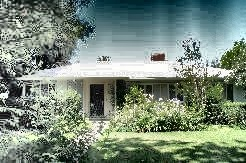
\includegraphics[width=0.45\textwidth]{./Figures/calhouse_230/0-resultado.jpg}
    }
%        \caption{Imagen Original. $\mathscr{H_Y}=0.207231$. $SSIM_R=1$. $SSIM_G=1$. $SSIM_B=1$}
\label{fig:calhouse2300}
\end{subfigure}
    ~ %add desired spacing between images. e. g. ~. \quad. \qquad. \hfill etc. 
      %(or a blank line to force the subfigure onto a new line)
      \begin{subfigure}[ID=1]{
      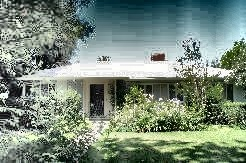
\includegraphics[width=0.45\textwidth]{./Figures/calhouse_230/1-resultado.jpg}   
      }
    %\begin{subfigure}[t]{0.45\textwidth}
%        \caption{Enhanced Image. $\mathscr{H_Y}=0.611275$. $SSIM_R=0.00897331$. $SSIM_G=0.00823064$. $SSIM_B=0.00851013$}
\label{fig:calhouse2301}
\end{subfigure}
    ~ %add desired spacing between images. e. g. ~. \quad. \qquad. \hfill etc. 
    %(or a blank line to force the subfigure onto a new line)
    \begin{subfigure}[ID=23]{
    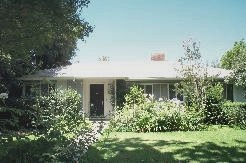
\includegraphics[width=0.45\textwidth]{./Figures/calhouse_230/23-resultado.jpg}
    }
    % \begin{subfigure}[t]{0.45\textwidth}
%        \caption{Enhanced Image.  $\mathscr{H_Y}=0.0350595$. $SSIM_R=0.416776$. $SSIM_G=0.403636$. $SSIM_B=0.417654$}
\label{fig:calhouse23023}
\end{subfigure} 
\begin{subfigure}[ID=24]{
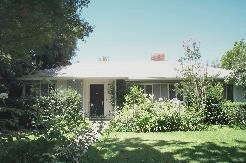
\includegraphics[width=0.45\textwidth]{./Figures/calhouse_230/24-resultado.jpg}
}
    % \begin{subfigure}[t]{0.45\textwidth}
        %\caption{Enhanced Image using \cite{morepso}. $\mathscr{H_Y}=0.788927$. $SSIM_R=0.000204143$. $SSIM_G=0.0000526475$. $SSIM_B=0.0000518143$}
        \label{fig:calhouse23024}
        \end{subfigure}
    ~ %add desired spacing between images. e. g. ~. \quad. \qquad. \hfill etc. 
    %(or a blank line to force the subfigure onto a new line)
    \begin{subfigure}[ID=56]{
    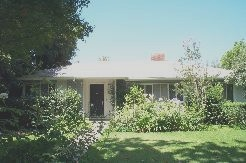
\includegraphics[width=0.45\textwidth]{./Figures/calhouse_230/56-resultado.jpg}
    }
    % \begin{subfigure}[t]{0.45\textwidth}
%        \caption{Enhanced Image.  $\mathscr{H_Y}=0.0350595$. $SSIM_R=0.416776$. $SSIM_G=0.403636$. $SSIM_B=0.417654$}
\label{fig:calhouse23056}
\end{subfigure} 
\begin{subfigure}[Imagen Original]{
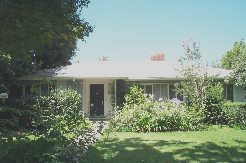
\includegraphics[width=0.45\textwidth]{./Figures/calhouse_230/calhouse_230.jpg}
}
    % \begin{subfigure}[t]{0.45\textwidth}
        %\caption{Enhanced Image using \cite{morepso}. $\mathscr{H_Y}=0.788927$. $SSIM_R=0.000204143$. $SSIM_G=0.0000526475$. $SSIM_B=0.0000518143$}
        \label{fig:calhouse230orig}
        \end{subfigure}
        \caption{Imágenes visualmente relevantes obtenidas mediante $CMOPSO-CLAHE$. Las variables y decisión y métricas de las imágenes se muestran en la tabla \ref{tab:calhouse_230}.}\label{fig:anexocalhouse230}
        \end{figure}

        \begin{figure}[H]
        \centering
        %\begin{subfigure}[Gráfica de Frente Pareto para las soluciones no dominadas de \texttt{calhouse_231.jpg}]{
        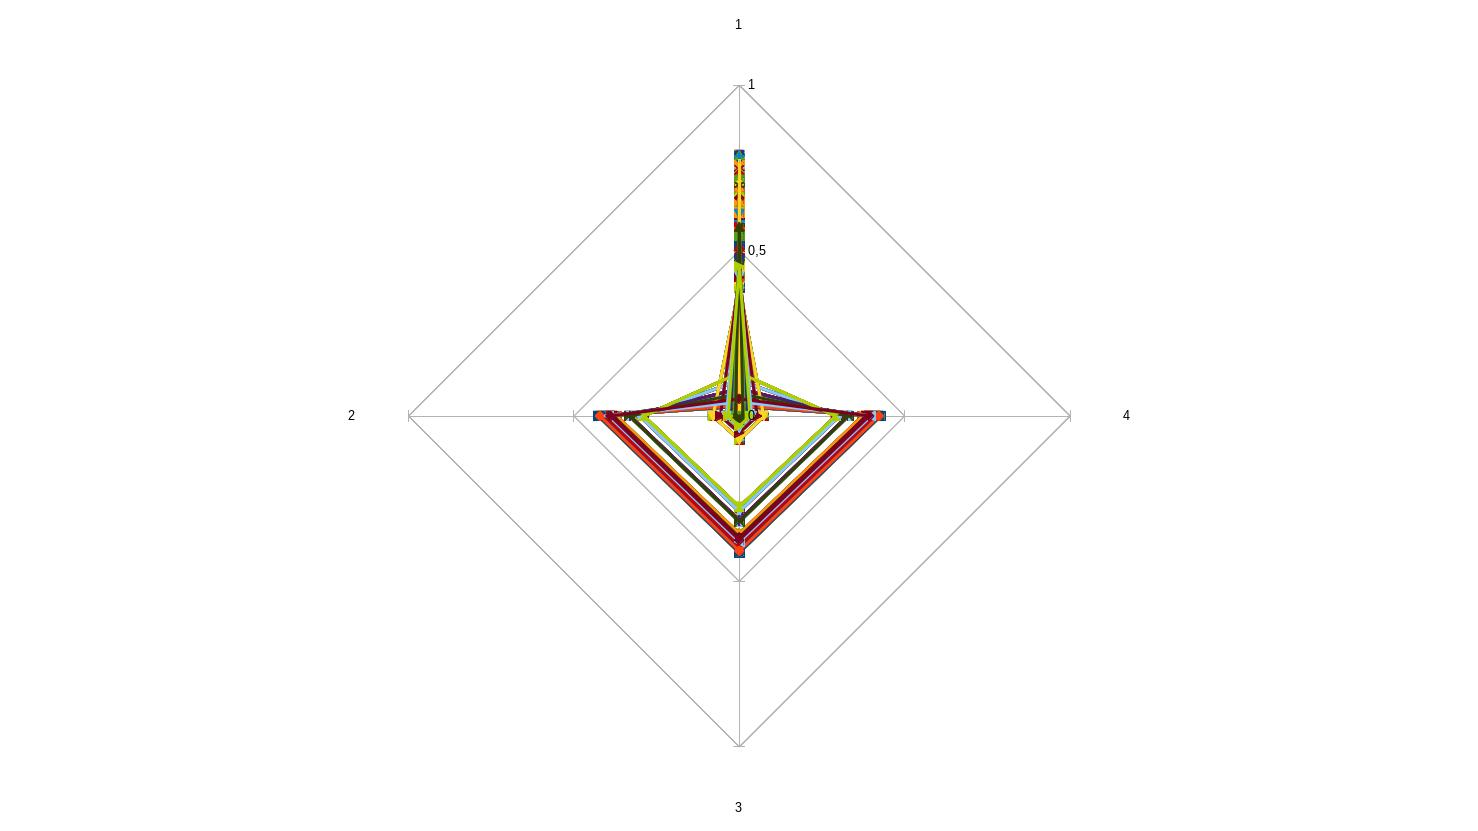
\includegraphics[width=\textwidth]{./Figures/calhouse_230/calhouse_230_2.jpg}
        %}
        %\end{subfigure}
        \caption{Frente pareto que contrasta los objetivos de las soluciones no dominadas. para los resultados de imágenes que se muestran en la tabla \ref{tab:calhouse_230}.}
        \label{fig:calhouse2302fp}
        \end{figure}


\section{Imagen de prueba \texttt{calhouse\_231.jpg}}

%calhouse 231
\scriptsize
\begin{longtable}{|c|c|c|c|c|c|c|c|}
% \centering
%\begin{tabular}
\hline
ID & $\mathscr{R}_x$ & $\mathscr{R}_y$ & $\mathscr{C}$ & $f_1(I.\vv{x})$ & $f_2(I.\vv{x})$ & $f_3(I.\vv{x})$ & $f_4(I.\vv{x})$ \\
0 & 18 & 3 & 0 & 0.00900173 & 0.267205 & 0.261971 & 0.266923 \\
1 & 13 & 2 & 0 & 0.00985956 & 0.259264 & 0.253973 & 0.258887 \\
2 & 10 & 2 & 0 & 0.00997639 & 0.256986 & 0.251503 & 0.256516 \\
3 & 10 & 2 & 0 & 0.0104213 & 0.255358 & 0.250056 & 0.255104 \\
4 & 8 & 2 & 0 & 0.0106044 & 0.253247 & 0.248009 & 0.252956 \\
5 & 8 & 2 & 0 & 0.0108852 & 0.248894 & 0.243521 & 0.248512 \\
6 & 5 & 3 & 0 & 0.0116286 & 0.242855 & 0.23726 & 0.242463 \\
7 & 37 & 2 & 0 & 0.0125856 & 0.204869 & 0.200071 & 0.20363 \\
8 & 18 & 2 & 0 & 0.012713 & 0.194229 & 0.189516 & 0.193111 \\
9 & 12 & 2 & 0 & 0.0130296 & 0.188019 & 0.183258 & 0.186758 \\
10 & 10 & 2 & 0 & 0.0133905 & 0.185665 & 0.180876 & 0.184348 \\
11 & 9 & 2 & 0 & 0.0134821 & 0.183211 & 0.178539 & 0.181995 \\
12 & 7 & 2 & 0 & 0.014287 & 0.177174 & 0.172057 & 0.1757 \\
13 & 5 & 2 & 0 & 0.0163016 & 0.174128 & 0.168903 & 0.172582 \\
14 & 4 & 2 & 0 & 0.0177784 & 0.168074 & 0.162957 & 0.166491 \\
15 & 3 & 2 & 0 & 0.0226231 & 0.1636 & 0.159053 & 0.162368 \\
16 & 2 & 2 & 0 & 0.026926 & 0.160205 & 0.156303 & 0.159384 \\
17 & 2 & 2 & 0 & 0.0431004 & 0.13865 & 0.136192 & 0.138648 \\
18 & 20 & 2 & 1 & 0.270889 & 0.0385879 & 0.0376327 & 0.0382134 \\
19 & 18 & 2 & 1 & 0.271006 & 0.0385725 & 0.0376188 & 0.0381991 \\
20 & 7 & 2 & 0.964079732103 & 0.276454 & 0.0381787 & 0.0368181 & 0.0376312 \\
21 & 2 & 2 & 0.989356928034 & 0.282013 & 0.038501 & 0.036779 & 0.0381451 \\
22 & 6 & 2 & 1 & 0.282743 & 0.0378731 & 0.0366182 & 0.0374679 \\
23 & 3 & 2 & 0.971840503575 & 0.284309 & 0.0371586 & 0.0357552 & 0.0367035 \\
24 & 4 & 2 & 0.972742419204 & 0.288689 & 0.0362972 & 0.0349026 & 0.0357714 \\
25 & 2 & 2 & 0.935457791487 & 0.289546 & 0.0364327 & 0.0347045 & 0.0360937 \\
26 & 2 & 2 & 0.940446088318 & 0.293769 & 0.0358847 & 0.0344679 & 0.0355097 \\
27 & 6 & 2 & 0.904740520538 & 0.295335 & 0.0347202 & 0.0334983 & 0.0342668 \\
28 & 9 & 2 & 1 & 0.298885 & 0.0334443 & 0.0324061 & 0.0330044 \\
29 & 14 & 2 & 1 & 0.299743 & 0.0334014 & 0.0323744 & 0.0329796 \\
30 & 10 & 2 & 0.913917022567 & 0.306106 & 0.0327387 & 0.0317938 & 0.032341 \\
31 & 12 & 2 & 1 & 0.307615 & 0.032043 & 0.0310592 & 0.0315852 \\
32 & 2 & 2 & 0.868629026061 & 0.309887 & 0.0325293 & 0.0309195 & 0.0322076 \\
33 & 7 & 2 & 0.922386499146 & 0.312944 & 0.0307703 & 0.0297033 & 0.0303923 \\
34 & 2 & 2 & 0.873918676927 & 0.314815 & 0.0305687 & 0.0293387 & 0.0302264 \\
35 & 12 & 2 & 0.828307512256 & 0.315595 & 0.029047 & 0.0281777 & 0.0286568 \\
36 & 7 & 2 & 0.90021573696 & 0.319267 & 0.0277445 & 0.0268512 & 0.0273699 \\
37 & 5 & 2 & 0.858598604984 & 0.325659 & 0.0279524 & 0.0268406 & 0.0275564 \\
38 & 6 & 2 & 0.856682527935 & 0.328166 & 0.0265695 & 0.0256397 & 0.0261868 \\
39 & 2 & 2 & 0.810611535096 & 0.333691 & 0.0265783 & 0.0254337 & 0.0262778 \\
40 & 14 & 2 & 0.826919288172 & 0.338436 & 0.0232717 & 0.0226148 & 0.0229894 \\
41 & 3 & 2 & 0.747934727522 & 0.354162 & 0.0228098 & 0.0218175 & 0.0225493 \\
42 & 2 & 2 & 0.715468922759 & 0.359465 & 0.0228153 & 0.0216203 & 0.0225292 \\
43 & 7 & 2 & 0.738152056945 & 0.362255 & 0.0220707 & 0.0212203 & 0.0216666 \\
44 & 5 & 2 & 0.710949498481 & 0.3623 & 0.0212484 & 0.0204049 & 0.0209322 \\
45 & 8 & 2 & 0.71860927648 & 0.365558 & 0.0191753 & 0.0185399 & 0.0188855 \\
46 & 17 & 2 & 0.638555526222 & 0.367131 & 0.0189012 & 0.0183635 & 0.0186746 \\
47 & 24 & 2 & 0.888901260944 & 0.372819 & 0.0186476 & 0.0180095 & 0.0183297 \\
48 & 7 & 2 & 0.643958573155 & 0.37555 & 0.0169599 & 0.0164014 & 0.016725 \\
49 & 5 & 2 & 0.627441542801 & 0.383322 & 0.0160663 & 0.0154653 & 0.0158211 \\
50 & 3 & 2 & 0.629994003473 & 0.391768 & 0.0161627 & 0.0153941 & 0.0159548 \\
51 & 19 & 2 & 0.545081379984 & 0.397269 & 0.0143794 & 0.0139211 & 0.0141685 \\
52 & 3 & 2 & 0.601135625969 & 0.402347 & 0.0145436 & 0.0138748 & 0.0143605 \\
53 & 3 & 2 & 0.57753934137 & 0.411112 & 0.013378 & 0.0127763 & 0.0131599 \\
54 & 2 & 2 & 0.541426023964 & 0.41398 & 0.0131499 & 0.0124833 & 0.0130018 \\
55 & 3 & 2 & 0.544335817577 & 0.414029 & 0.0125525 & 0.0119757 & 0.0123731 \\
56 & 6 & 2 & 0.548121706633 & 0.414094 & 0.0120755 & 0.0115387 & 0.0117838 \\
57 & 2 & 2 & 0.515852425305 & 0.421322 & 0.011292 & 0.010746 & 0.0111554 \\
58 & 31 & 2 & 0.0280991811699 & 0.423455 & 0.0107604 & 0.0102737 & 0.010496 \\
59 & 33 & 2 & 0.510626077249 & 0.42346 & 0.0107601 & 0.0102734 & 0.0104956 \\
60 & 3 & 2 & 0.5 & 0.426877 & 0.0107589 & 0.0102665 & 0.0106218 \\
61 & 9 & 2 & 0.5 & 0.428904 & 0.0107733 & 0.0101945 & 0.0103729 \\
62 & 13 & 2 & 0.5 & 0.431454 & 0.00965356 & 0.00927182 & 0.0094467 \\
63 & 7 & 2 & 0.478914771532 & 0.435993 & 0.00828631 & 0.00795353 & 0.00813127 \\
64 & 5 & 2 & 0.457071559114 & 0.442431 & 0.00817965 & 0.00780437 & 0.0080066 \\
65 & 2 & 2 & 0.429496349756 & 0.446127 & 0.00810596 & 0.00772429 & 0.00801587 \\
66 & 3 & 2 & 0.442489234125 & 0.447001 & 0.00778622 & 0.00745209 & 0.00769754 \\
67 & 9 & 2 & 0.456539353563 & 0.45027 & 0.00668378 & 0.00648114 & 0.00659949 \\
68 & 5 & 2 & 0.376465221858 & 0.456932 & 0.00627423 & 0.00605903 & 0.00619215 \\
69 & 8 & 2 & 0.461600206088 & 0.460667 & 0.00621708 & 0.00592585 & 0.00603826 \\
70 & 8 & 2 & 0.360353977865 & 0.462861 & 0.00579699 & 0.00562394 & 0.00572817 \\
71 & 2 & 5 & 0.411676225675 & 0.471886 & 0.00573421 & 0.00559339 & 0.0057057 \\
72 & 3 & 2 & 0.372641778915 & 0.475316 & 0.00536055 & 0.00515606 & 0.00529048 \\
73 & 8 & 2 & 0.399775248471 & 0.475386 & 0.00529207 & 0.00510996 & 0.00520481 \\
74 & 3 & 2 & 0.339070248196 & 0.47558 & 0.00452605 & 0.004307 & 0.00443858 \\
75 & 4 & 2 & 0.351684592681 & 0.479774 & 0.00435225 & 0.00410036 & 0.00418851 \\
76 & 4 & 2 & 0.349489075978 & 0.482928 & 0.00426761 & 0.00405113 & 0.00415045 \\
77 & 3 & 2 & 0.337330254689 & 0.488762 & 0.00401598 & 0.00385289 & 0.00397122 \\
78 & 2 & 2 & 0.30899847401 & 0.491558 & 0.00390371 & 0.00373161 & 0.00387131 \\
79 & 2 & 9 & 0.278605575898 & 0.49243 & 0.00331112 & 0.00334138 & 0.00338704 \\
80 & 2 & 2 & 0.309171129718 & 0.49718 & 0.00289651 & 0.00277638 & 0.00282767 \\
81 & 2 & 9 & 0.22375153796 & 0.499764 & 0.00285511 & 0.00284174 & 0.0028875 \\
82 & 3 & 2 & 0.300745369259 & 0.506126 & 0.00229212 & 0.00217746 & 0.00221458 \\
83 & 4 & 2 & 0.263406661906 & 0.506628 & 0.00222147 & 0.00211851 & 0.00215494 \\
84 & 2 & 2 & 0.251424143589 & 0.513605 & 0.00194255 & 0.00184685 & 0.00190236 \\
85 & 5 & 2 & 0.243696919714 & 0.514978 & 0.00176819 & 0.00169965 & 0.00173187 \\
86 & 4 & 2 & 0.209648277039 & 0.516483 & 0.00166633 & 0.0015921 & 0.00162961 \\
87 & 4 & 3 & 0.266234136177 & 0.520381 & 0.00166707 & 0.00158428 & 0.0016109 \\
88 & 2 & 4 & 0.248121384745 & 0.521675 & 0.00161956 & 0.00153988 & 0.00158018 \\
89 & 3 & 2 & 0.213491461803 & 0.525156 & 0.00144721 & 0.00138333 & 0.00141691 \\
90 & 2 & 2 & 0.191537420599 & 0.52922 & 0.00135061 & 0.00127997 & 0.00130769 \\
91 & 3 & 2 & 0.183704209136 & 0.530389 & 0.00119938 & 0.00115064 & 0.00116924 \\
92 & 2 & 3 & 0.178720787449 & 0.534519 & 0.00114637 & 0.00109067 & 0.00111032 \\
93 & 7 & 2 & 0.241533503656 & 0.536006 & 0.00110823 & 0.00103223 & 0.00105307 \\
94 & 2 & 2 & 0.167767741924 & 0.540966 & 0.000784735 & 0.000735661 & 0.000749385 \\
95 & 2 & 3 & 0.165303683073 & 0.546799 & 0.000724879 & 0.000653544 & 0.000674347 \\
96 & 2 & 2 & 0.14568920398 & 0.549775 & 0.00055956 & 0.00050608 & 0.000516374 \\
97 & 2 & 7 & 0.0971302704582 & 0.551463 & 0.0005087 & 0.000484928 & 0.000491999 \\
98 & 3 & 4 & 0.0169016006744 & 0.55715 & 0.000453264 & 0.000428699 & 0.000432725 \\
99 & 2 & 3 & 0.0764136259071 & 0.561146 & 0.000201883 & 0.000166411 & 0.000174052 \\
100 & 2 & 2 & 0.049662954082 & 0.565069 & 0.000189286 & 0.000165373 & 0.000167802 \\
101 & 3 & 3 & 0.0412250071562 & 0.573604 & 0.000167373 & 0.000136933 & 0.000144334 \\
102 & 2 & 2 & 0.0213381170565 & 0.573629 & 0.000103816 & 7.68E-05 & 7.86E-05 \\
\hline
\multicolumn{8}{|c|}{\textbf{Tiempos de ejecución:} \texttt{real:70m26.492s. user:209m3.921s. sys:95m37.357s}}\\  \hline
% \end{tabular}
\caption{Resultados no dominados para la imagen de prueba \texttt{calhouse\_231.jpg}}
\label{tab:calhouse_231}
\end{longtable}
\normalsize

\begin{figure}[H]
\centering
    %\begin{subfigure}[t]{0.45\textwidth}
    \begin{subfigure}[ID=0]{
    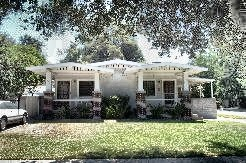
\includegraphics[width=0.45\textwidth]{./Figures/calhouse_231/0-resultado.jpg}
    }
%        \caption{Imagen Original. $\mathscr{H_Y}=0.207231$. $SSIM_R=1$. $SSIM_G=1$. $SSIM_B=1$}
\label{fig:calhouse2310}
\end{subfigure}
    ~ %add desired spacing between images. e. g. ~. \quad. \qquad. \hfill etc. 
      %(or a blank line to force the subfigure onto a new line)
      \begin{subfigure}[ID=1]{
      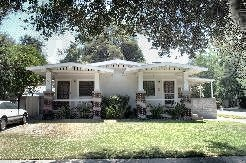
\includegraphics[width=0.45\textwidth]{./Figures/calhouse_231/1-resultado.jpg}   
      }
    %\begin{subfigure}[t]{0.45\textwidth}
%        \caption{Enhanced Image. $\mathscr{H_Y}=0.611275$. $SSIM_R=0.00897331$. $SSIM_G=0.00823064$. $SSIM_B=0.00851013$}
\label{fig:calhouse2311}
\end{subfigure}
    ~ %add desired spacing between images. e. g. ~. \quad. \qquad. \hfill etc. 
    %(or a blank line to force the subfigure onto a new line)
    \begin{subfigure}[ID=23]{
    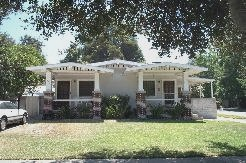
\includegraphics[width=0.45\textwidth]{./Figures/calhouse_231/28-resultado.jpg}
    }
    % \begin{subfigure}[t]{0.45\textwidth}
%        \caption{Enhanced Image.  $\mathscr{H_Y}=0.0350595$. $SSIM_R=0.416776$. $SSIM_G=0.403636$. $SSIM_B=0.417654$}
\label{fig:calhouse23128}
\end{subfigure} 
\begin{subfigure}[ID=24]{
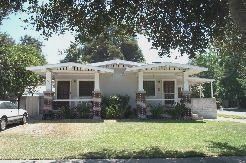
\includegraphics[width=0.45\textwidth]{./Figures/calhouse_231/29-resultado.jpg}
}
    % \begin{subfigure}[t]{0.45\textwidth}
        %\caption{Enhanced Image using \cite{morepso}. $\mathscr{H_Y}=0.788927$. $SSIM_R=0.000204143$. $SSIM_G=0.0000526475$. $SSIM_B=0.0000518143$}
        \label{fig:calhouse23129}
        \end{subfigure}
    ~ %add desired spacing between images. e. g. ~. \quad. \qquad. \hfill etc. 
    %(or a blank line to force the subfigure onto a new line)
    \begin{subfigure}[ID=56]{
    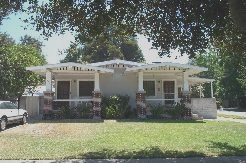
\includegraphics[width=0.45\textwidth]{./Figures/calhouse_231/102-resultado.jpg}
    }
    % \begin{subfigure}[t]{0.45\textwidth}
%        \caption{Enhanced Image.  $\mathscr{H_Y}=0.0350595$. $SSIM_R=0.416776$. $SSIM_G=0.403636$. $SSIM_B=0.417654$}
\label{fig:calhouse231102}
\end{subfigure} 
\begin{subfigure}[Imagen Original]{
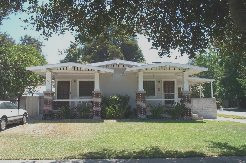
\includegraphics[width=0.45\textwidth]{./Figures/calhouse_231/calhouse_231.jpg}
}
    % \begin{subfigure}[t]{0.45\textwidth}
        %\caption{Enhanced Image using \cite{morepso}. $\mathscr{H_Y}=0.788927$. $SSIM_R=0.000204143$. $SSIM_G=0.0000526475$. $SSIM_B=0.0000518143$}
        \label{fig:calhouse231orig}
        \end{subfigure}
        \caption{Imágenes visualmente relevantes obtenidas mediante $CMOPSO-CLAHE$. Las variables y decisión y métricas de las imágenes se muestran en la tabla \ref{tab:calhouse_231}.}
        \label{fig:anexocalhouse230}
        \end{figure}

        \begin{figure}[H]
        \centering
        %\begin{subfigure}[Gráfica de Frente Pareto para las soluciones no dominadas de \texttt{calhouse_231.jpg}]{
        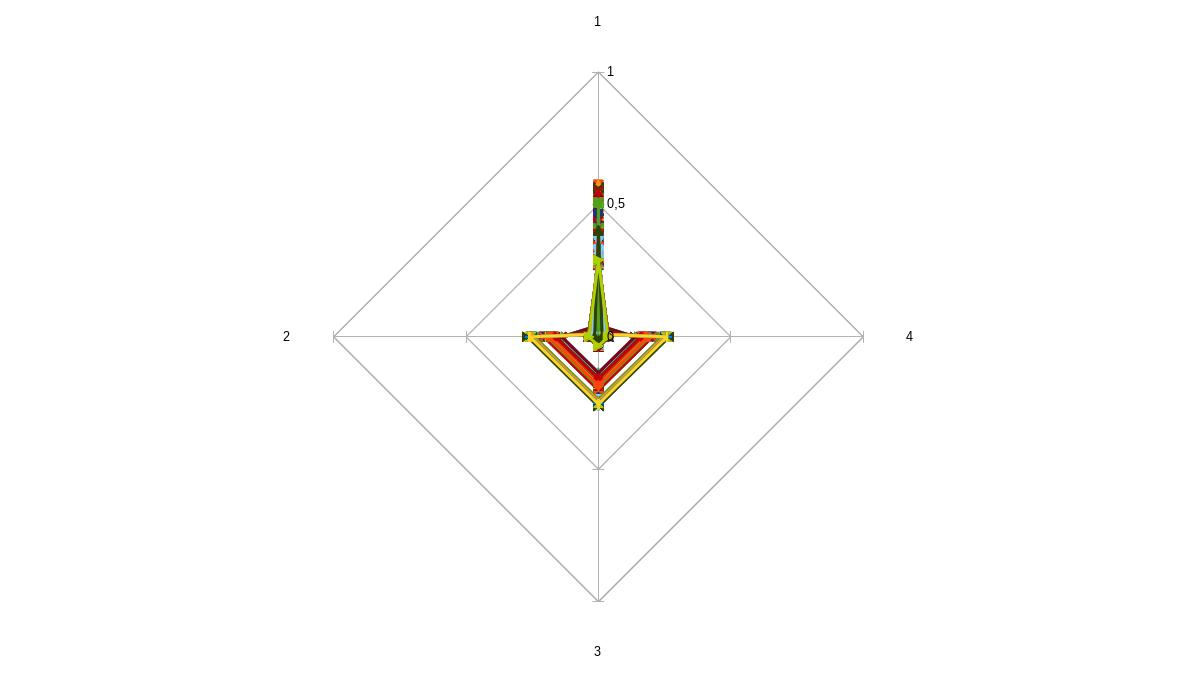
\includegraphics[width=\textwidth]{./Figures/calhouse_231/calhouse_231_2.jpg}
        %}
        %\end{subfigure}
        \caption{Frente pareto que contrasta los objetivos de las soluciones no dominadas. para los resultados de imágenes que se muestran en la tabla \ref{tab:calhouse_231}.}
        \label{fig:calhouse2312fp}
        \end{figure}

\section{Imagen de prueba \texttt{calhouse\_233.jpg}}

%calhouse 231
\scriptsize
\begin{longtable}{|c|c|c|c|c|c|c|c|}
% \centering
%\begin{tabular}
\hline
ID & $\mathscr{R}_x$ & $\mathscr{R}_y$ & $\mathscr{C}$ & $f_1(I.\vv{x})$ & $f_2(I.\vv{x})$ & $f_3(I.\vv{x})$ & $f_4(I.\vv{x})$ \\
0 & 4 & 2 & 0.0605454359216 & 1.08964 & 0.000295689 & 0.000153393 & 0.000162248 \\
1 & 2 & 3 & 0.0241100460642 & 1.05839 & 0.000302083 & 0.000187229 & 0.00018095 \\
2 & 3 & 2 & 0.0755634120675 & 1.08786 & 0.000329964 & 0.000184893 & 0.000199624 \\
3 & 2 & 6 & 0.0362807189867 & 1.03646 & 0.000641662 & 0.000514385 & 0.000524924 \\
4 & 8 & 3 & 0.103753483353 & 1.03239 & 0.00102858 & 0.000843436 & 0.000877847 \\
5 & 2 & 3 & 0.166601922869 & 0.993392 & 0.00117745 & 0.00100106 & 0.00102251 \\
6 & 4 & 3 & 0.197035454701 & 0.972543 & 0.00121931 & 0.00104515 & 0.00106603 \\
7 & 2 & 3 & 0.232499530296 & 0.95589 & 0.00235641 & 0.002009 & 0.00206351 \\
8 & 2 & 5 & 0.266574790017 & 0.938972 & 0.00280239 & 0.00262648 & 0.0026463 \\
9 & 2 & 3 & 0.278743476534 & 0.923925 & 0.00292607 & 0.00257795 & 0.00266449 \\
10 & 3 & 4 & 0.278646550346 & 0.92028 & 0.00292439 & 0.00261397 & 0.00266665 \\
11 & 12 & 3 & 0.30091560684 & 0.870766 & 0.00350392 & 0.00310311 & 0.00316902 \\
12 & 2 & 4 & 0.253592839376 & 0.919652 & 0.00348043 & 0.00316849 & 0.00322916 \\
13 & 2 & 3 & 0.391124890124 & 0.864988 & 0.00550206 & 0.00480986 & 0.00499557 \\
14 & 2 & 4 & 0.35510717405 & 0.830931 & 0.00598392 & 0.00560268 & 0.0056997 \\
15 & 16 & 3 & 0.227910808421 & 0.826457 & 0.00687623 & 0.00604448 & 0.00619402 \\
16 & 8 & 3 & 0.450962738883 & 0.819552 & 0.00842425 & 0.0076944 & 0.00785632 \\
17 & 5 & 3 & 0.5 & 0.810249 & 0.00887391 & 0.00800675 & 0.00821064 \\
18 & 2 & 3 & 0.534064898653 & 0.798087 & 0.0102274 & 0.00910215 & 0.00944354 \\
19 & 5 & 3 & 0.571647250785 & 0.785827 & 0.011758 & 0.0105297 & 0.010857 \\
20 & 2 & 4 & 0.506882563198 & 0.778071 & 0.0115198 & 0.0108465 & 0.0110746 \\
21 & 2 & 3 & 0.609611782643 & 0.763786 & 0.0131498 & 0.0117422 & 0.0121901 \\
22 & 3 & 4 & 0.590722339759 & 0.770255 & 0.0127545 & 0.0120351 & 0.0122763 \\
23 & 2 & 4 & 0.592771396022 & 0.759783 & 0.0134854 & 0.0128619 & 0.0130943 \\
24 & 10 & 3 & 0.569430012343 & 0.753103 & 0.0148294 & 0.0134841 & 0.0137764 \\
25 & 2 & 3 & 0.654795564549 & 0.758248 & 0.0146595 & 0.013324 & 0.0137805 \\
26 & 23 & 3 & 0.49018750213 & 0.745152 & 0.0156444 & 0.0140341 & 0.0143124 \\
27 & 5 & 3 & 0.711411054066 & 0.75186 & 0.0155433 & 0.0142944 & 0.0146168 \\
28 & 6 & 3 & 0.67594979599 & 0.742439 & 0.016272 & 0.014948 & 0.0152924 \\
29 & 3 & 3 & 0.697388429306 & 0.740592 & 0.0161852 & 0.0148598 & 0.015301 \\
30 & 2 & 4 & 0.619064681832 & 0.721047 & 0.0169986 & 0.0162408 & 0.0165372 \\
31 & 12 & 3 & 0.758015111952 & 0.715111 & 0.0179455 & 0.0167202 & 0.0170063 \\
32 & 2 & 4 & 0.664983118922 & 0.717893 & 0.018933 & 0.018076 & 0.0184091 \\
33 & 3 & 3 & 0.835945114263 & 0.715581 & 0.0212394 & 0.0197281 & 0.0202355 \\
34 & 18 & 4 & 0.235751993872 & 0.71698 & 0.0217524 & 0.0198408 & 0.0203643 \\
35 & 2 & 4 & 0.71221653662 & 0.697186 & 0.0211379 & 0.0202178 & 0.0205842 \\
36 & 3 & 3 & 0.841409534625 & 0.694649 & 0.024789 & 0.0230342 & 0.0236651 \\
37 & 2 & 4 & 0.775805262395 & 0.690287 & 0.0242775 & 0.023289 & 0.0236959 \\
38 & 6 & 3 & 0.946937444304 & 0.688181 & 0.027246 & 0.025366 & 0.0259008 \\
39 & 3 & 3 & 0.898145960419 & 0.688406 & 0.027186 & 0.0254119 & 0.0260424 \\
40 & 8 & 3 & 0.92952634183 & 0.682212 & 0.027619 & 0.026095 & 0.0265493 \\
41 & 2 & 3 & 0.92681679413 & 0.664923 & 0.0280842 & 0.0260755 & 0.0268696 \\
42 & 2 & 4 & 0.831514829931 & 0.682197 & 0.0278131 & 0.0267008 & 0.0271825 \\
43 & 3 & 3 & 1 & 0.662133 & 0.0302244 & 0.0283526 & 0.0290769 \\
44 & 2 & 3 & 1 & 0.638068 & 0.0319237 & 0.0297923 & 0.0307026 \\
45 & 44 & 3 & 0.340457573545 & 0.597537 & 0.0430642 & 0.0399363 & 0.0405722 \\
46 & 41 & 4 & 0.122685175212 & 0.585286 & 0.0791404 & 0.0724312 & 0.0744605 \\
47 & 2 & 2 & 0 & 0.166749 & 0.35221 & 0.33188 & 0.347256 \\
48 & 3 & 2 & 0 & 0.162343 & 0.36439 & 0.343949 & 0.35654 \\
49 & 4 & 2 & 0 & 0.0834117 & 0.383713 & 0.363361 & 0.373847 \\
50 & 5 & 2 & 0 & 0.0629735 & 0.391495 & 0.37163 & 0.381356 \\
51 & 11 & 2 & 0 & 0.0619745 & 0.418598 & 0.398414 & 0.406889 \\
52 & 26 & 2 & 0 & 0.0599365 & 0.437032 & 0.417224 & 0.424583 \\
53 & 6 & 3 & 0 & 0.0475216 & 0.459573 & 0.445796 & 0.456496 \\
54 & 9 & 3 & 0 & 0.0462856 & 0.470122 & 0.456474 & 0.466522 \\
55 & 11 & 3 & 0 & 0.0443048 & 0.475939 & 0.462247 & 0.471704 \\
56 & 2 & 6 & 0 & 0.0455046 & 0.470176 & 0.461747 & 0.47771 \\
57 & 2 & 7 & 0 & 0.0444002 & 0.493213 & 0.484229 & 0.499757 \\
58 & 2 & 9 & 0 & 0.0408697 & 0.499463 & 0.490757 & 0.507241 \\
59 & 2 & 10 & 0 & 0.0359039 & 0.511722 & 0.502448 & 0.518851 \\
60 & 2 & 2 & 0.00447401966895 & 1.09149 & 0.000183402 & 7.05E-05 & 6.21E-05 \\
\hline
\multicolumn{8}{|c|}{\textbf{Tiempos de ejecución:} \texttt{real:67m22.885s.user:207m13.352s.sys:94m57.439s
}}\\  \hline
% \end{tabular}
\caption{Resultados no dominados para la imagen de prueba \texttt{calhouse\_233.jpg}}
\label{tab:calhouse_233}
\end{longtable}
\normalsize

\begin{figure}[H]
\centering
    %\begin{subfigure}[t]{0.45\textwidth}
    \begin{subfigure}[ID=0]{
    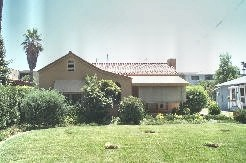
\includegraphics[width=0.45\textwidth]{./Figures/calhouse_233/6-resultado.jpg}
    }
%        \caption{Imagen Original. $\mathscr{H_Y}=0.207231$. $SSIM_R=1$. $SSIM_G=1$. $SSIM_B=1$}
\end{subfigure}
    ~ %add desired spacing between images. e. g. ~. \quad. \qquad. \hfill etc. 
      %(or a blank line to force the subfigure onto a new line)
      \begin{subfigure}[ID=1]{
      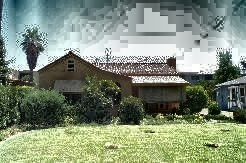
\includegraphics[width=0.45\textwidth]{./Figures/calhouse_233/7-resultado.jpg}   
      }
    %\begin{subfigure}[t]{0.45\textwidth}
%        \caption{Enhanced Image. $\mathscr{H_Y}=0.611275$. $SSIM_R=0.00897331$. $SSIM_G=0.00823064$. $SSIM_B=0.00851013$}
\end{subfigure}
    ~ %add desired spacing between images. e. g. ~. \quad. \qquad. \hfill etc. 
    %(or a blank line to force the subfigure onto a new line)
    \begin{subfigure}[ID=23]{
    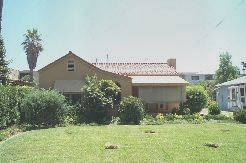
\includegraphics[width=0.45\textwidth]{./Figures/calhouse_233/46-resultado.jpg}
    }
    % \begin{subfigure}[t]{0.45\textwidth}
%        \caption{Enhanced Image.  $\mathscr{H_Y}=0.0350595$. $SSIM_R=0.416776$. $SSIM_G=0.403636$. $SSIM_B=0.417654$}
\end{subfigure} 
\begin{subfigure}[ID=24]{
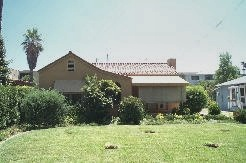
\includegraphics[width=0.45\textwidth]{./Figures/calhouse_233/47-resultado.jpg}
}
    % \begin{subfigure}[t]{0.45\textwidth}
        %\caption{Enhanced Image using \cite{morepso}. $\mathscr{H_Y}=0.788927$. $SSIM_R=0.000204143$. $SSIM_G=0.0000526475$. $SSIM_B=0.0000518143$}
        \label{fig:calhouse23129}
        \end{subfigure}
    ~ %add desired spacing between images. e. g. ~. \quad. \qquad. \hfill etc. 
    %(or a blank line to force the subfigure onto a new line)
    \begin{subfigure}[ID=56]{
    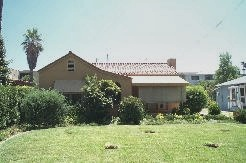
\includegraphics[width=0.45\textwidth]{./Figures/calhouse_233/60-resultado.jpg}
    }
    % \begin{subfigure}[t]{0.45\textwidth}
%        \caption{Enhanced Image.  $\mathscr{H_Y}=0.0350595$. $SSIM_R=0.416776$. $SSIM_G=0.403636$. $SSIM_B=0.417654$}
\label{fig:calhouse231102}
\end{subfigure} 
\begin{subfigure}[Imagen Original]{
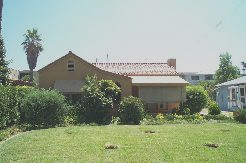
\includegraphics[width=0.45\textwidth]{./Figures/calhouse_233/calhouse_233.jpg}
}
    % \begin{subfigure}[t]{0.45\textwidth}
        %\caption{Enhanced Image using \cite{morepso}. $\mathscr{H_Y}=0.788927$. $SSIM_R=0.000204143$. $SSIM_G=0.0000526475$. $SSIM_B=0.0000518143$}
        \label{fig:calhouse233orig}
        \end{subfigure}
        \caption{Imágenes visualmente relevantes obtenidas mediante $CMOPSO-CLAHE$. Las variables y decisión y métricas de las imágenes se muestran en la tabla \ref{tab:calhouse_233}.}
        \label{fig:anexocalhouse233}
        \end{figure}

        \begin{figure}[H]
        \centering
        %\begin{subfigure}[Gráfica de Frente Pareto para las soluciones no dominadas de \texttt{calhouse_231.jpg}]{
        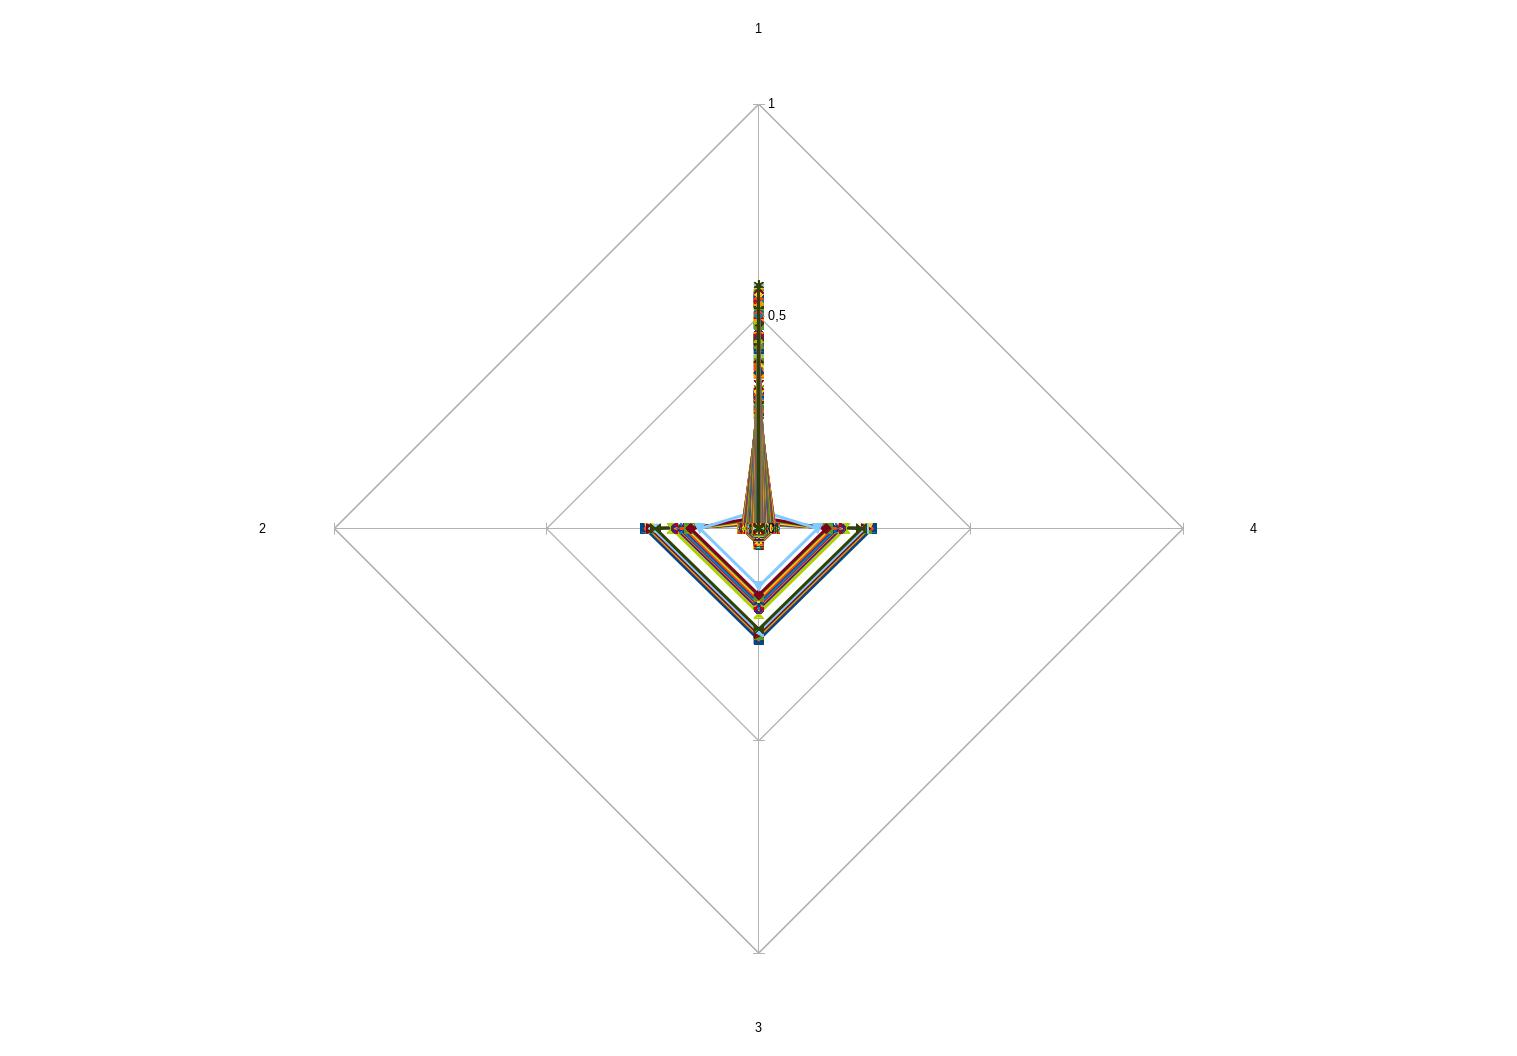
\includegraphics[width=\textwidth]{./Figures/calhouse_233/calhouse_233_2.jpg}
        %}
        %\end{subfigure}
        \caption{Frente pareto que contrasta los objetivos de las soluciones no dominadas. para los resultados de imágenes que se muestran en la tabla \ref{tab:calhouse_233}.}
        \label{fig:calhouse2332fp}
        \end{figure}


\section{Imagen de prueba \texttt{calhouse\_234.jpg}}

%calhouse 234
\scriptsize
\begin{longtable}{|c|c|c|c|c|c|c|c|}
% \centering
%\begin{tabular}
\hline
ID & $\mathscr{R}_x$ & $\mathscr{R}_y$ & $\mathscr{C}$ & $f_1(I.\vv{x})$ & $f_2(I.\vv{x})$ & $f_3(I.\vv{x})$ & $f_4(I.\vv{x})$ \\
2979 & 3 & 3 & 0.812519298752 & 0.511109 & 0.0287218 & 0.0274117 & 0.0284403 \\
2980 & 4 & 12 & 0 & 0.0276203 & 0.49051 & 0.486184 & 0.493034 \\
3091 & 4 & 2 & 0.853706507459 & 0.519737 & 0.027535 & 0.0255765 & 0.0267492 \\
3097 & 11 & 2 & 1 & 0.494054 & 0.034029 & 0.032038 & 0.0331011 \\
3104 & 20 & 3 & 0 & 0.0284328 & 0.402012 & 0.396043 & 0.401629 \\
3123 & 3 & 3 & 0.739306706876 & 0.533226 & 0.024867 & 0.0237548 & 0.0245899 \\
3125 & 2 & 2 & 0.731703535828 & 0.548753 & 0.0229975 & 0.0211807 & 0.0222653 \\
3126 & 3 & 2 & 0.679146848174 & 0.557746 & 0.0203147 & 0.0187927 & 0.0196922 \\
3127 & 2 & 2 & 0.850344549266 & 0.515146 & 0.029663 & 0.0272264 & 0.0286435 \\
3128 & 14 & 2 & 0.632770576643 & 0.58597 & 0.01286 & 0.0122675 & 0.0126854 \\
3129 & 53 & 3 & 0.0906614748552 & 0.41236 & 0.10348 & 0.0946411 & 0.0973958 \\
3130 & 8 & 2 & 0.368264089891 & 0.675727 & 0.00441494 & 0.00421142 & 0.00434589 \\
3131 & 2 & 2 & 0.827779089761 & 0.524632 & 0.0281598 & 0.0258405 & 0.0271833 \\
3132 & 2 & 2 & 0 & 0.138669 & 0.231124 & 0.221532 & 0.228493 \\
3133 & 37 & 4 & 0.488860216273 & 0.445821 & 0.0866204 & 0.0792098 & 0.0816776 \\
3134 & 4 & 2 & 0.255668440752 & 0.730788 & 0.00268251 & 0.00253008 & 0.00260924 \\
3135 & 6 & 2 & 0.912272466777 & 0.496642 & 0.0326795 & 0.0303633 & 0.0316357 \\
3136 & 2 & 2 & 0.0083970078807 & 0.835548 & 0.000142314 & 0.000115598 & 0.000110237 \\
3137 & 3 & 2 & 0.461160630083 & 0.650707 & 0.00852852 & 0.00796836 & 0.00830184 \\
3138 & 3 & 2 & 0.73164070769 & 0.551425 & 0.0215359 & 0.0198995 & 0.0208231 \\
3139 & 4 & 2 & 0.0653533397144 & 0.832464 & 0.000183395 & 0.000143403 & 0.000147903 \\
3140 & 3 & 2 & 0.148486630518 & 0.793742 & 0.000731432 & 0.000664557 & 0.000679274 \\
3141 & 18 & 2 & 0.572302594831 & 0.62303 & 0.00889421 & 0.00828233 & 0.00854233 \\
3142 & 13 & 3 & 0 & 0.0292034 & 0.390222 & 0.383769 & 0.389344 \\
3143 & 9 & 2 & 0.515175605936 & 0.640419 & 0.00871692 & 0.00817691 & 0.00844283 \\
3144 & 10 & 2 & 0.645449480383 & 0.580588 & 0.0168114 & 0.0159317 & 0.0165228 \\
3145 & 24 & 3 & 0 & 0.0277634 & 0.406696 & 0.400567 & 0.40603 \\
3146 & 6 & 2 & 0 & 0.0493283 & 0.277246 & 0.269315 & 0.27368 \\
3147 & 2 & 2 & 0.761261125963 & 0.54257 & 0.0246297 & 0.0226156 & 0.0237819 \\
3148 & 5 & 2 & 0 & 0.0519104 & 0.273498 & 0.265907 & 0.270653 \\
3149 & 2 & 2 & 0.926215684557 & 0.493326 & 0.0350073 & 0.032038 & 0.0337141 \\
3150 & 5 & 3 & 0.907757451731 & 0.507807 & 0.0309136 & 0.0296258 & 0.0305795 \\
3151 & 2 & 2 & 0.729074889936 & 0.553606 & 0.021385 & 0.0196689 & 0.0206698 \\
3152 & 3 & 2 & 0 & 0.0846047 & 0.245215 & 0.237309 & 0.244065 \\
3153 & 3 & 2 & 0.854113478667 & 0.512472 & 0.030045 & 0.027703 & 0.0290506 \\
3154 & 7 & 3 & 0 & 0.0321503 & 0.363205 & 0.357271 & 0.362161 \\
3155 & 24 & 2 & 1 & 0.448877 & 0.0337654 & 0.0325268 & 0.0334449 \\
3156 & 4 & 2 & 0.780918170773 & 0.530471 & 0.0249754 & 0.0230687 & 0.0241613 \\
3157 & 6 & 2 & 0.196390542599 & 0.78611 & 0.000841764 & 0.00080091 & 0.000816869 \\
3158 & 2 & 3 & 0.833866902733 & 0.511989 & 0.0302699 & 0.0285167 & 0.0297871 \\
3159 & 6 & 2 & 0.747192629244 & 0.547824 & 0.0229913 & 0.0213657 & 0.0222196 \\
3160 & 3 & 2 & 0.80975515976 & 0.527355 & 0.0266691 & 0.0245697 & 0.0257519 \\
3161 & 7 & 2 & 0 & 0.0413656 & 0.289774 & 0.282049 & 0.285934 \\
3162 & 3 & 3 & 0.725942475481 & 0.553035 & 0.0211689 & 0.0201818 & 0.0209119 \\
3163 & 2 & 3 & 0.0869925259854 & 0.831217 & 0.000254231 & 0.000202246 & 0.000220666 \\
3164 & 3 & 2 & 0.101165992212 & 0.829471 & 0.000258416 & 0.000220973 & 0.000231715 \\
3165 & 6 & 2 & 0.846937821181 & 0.518807 & 0.027765 & 0.0259249 & 0.0270216 \\
3166 & 3 & 2 & 0.305290000047 & 0.710093 & 0.00364066 & 0.0034385 & 0.00355669 \\
3167 & 11 & 2 & 0 & 0.0396638 & 0.306313 & 0.297956 & 0.302221 \\
3168 & 7 & 2 & 0.219179192327 & 0.773407 & 0.00121588 & 0.00114323 & 0.00117378 \\
3169 & 5 & 2 & 0.227660930211 & 0.738358 & 0.00171736 & 0.0016441 & 0.00168794 \\
3170 & 26 & 6 & 0.511796994819 & 0.445776 & 0.0921568 & 0.0871899 & 0.0896835 \\
3171 & 3 & 2 & 0.225128485738 & 0.755389 & 0.00142469 & 0.00136878 & 0.00139945 \\
3172 & 2 & 3 & 0.0112353502775 & 0.836594 & 0.000146742 & 0.000117982 & 0.000110062 \\
3173 & 17 & 2 & 0.73226869704 & 0.574325 & 0.0167192 & 0.0159348 & 0.0164249 \\
3174 & 11 & 3 & 0 & 0.0296307 & 0.381211 & 0.374829 & 0.380207 \\
3175 & 4 & 2 & 0.863033788718 & 0.502655 & 0.0311266 & 0.0287067 & 0.03005 \\
3176 & 14 & 2 & 0.937018260677 & 0.502234 & 0.0314391 & 0.0298899 & 0.0308901 \\
3177 & 3 & 3 & 0.578272628825 & 0.582351 & 0.0151525 & 0.0144716 & 0.0149766 \\
3178 & 6 & 2 & 0.682234104882 & 0.564373 & 0.0195332 & 0.0183163 & 0.019096 \\
3179 & 18 & 2 & 0.783902002406 & 0.533793 & 0.0238637 & 0.022623 & 0.0232914 \\
3180 & 4 & 3 & 0.403556720027 & 0.65922 & 0.00689137 & 0.00665012 & 0.00686885 \\
3181 & 2 & 3 & 0.885217278433 & 0.492458 & 0.0341363 & 0.0321934 & 0.0336531 \\
3182 & 11 & 2 & 0.317936251338 & 0.723333 & 0.00331185 & 0.00315496 & 0.00324682 \\
3183 & 15 & 2 & 0.5 & 0.666303 & 0.00554846 & 0.00524035 & 0.00540413 \\
3184 & 12 & 2 & 0.522610271857 & 0.601996 & 0.0103419 & 0.00983332 & 0.010186 \\
3185 & 11 & 2 & 0.95 & 0.513048 & 0.0288726 & 0.0272513 & 0.0282724 \\
3186 & 3 & 3 & 0.656165744218 & 0.571977 & 0.0180757 & 0.0172713 & 0.0179017 \\
3187 & 13 & 2 & 0.956428228721 & 0.524695 & 0.0260812 & 0.024745 & 0.0255167 \\
\hline
\multicolumn{8}{|c|}{\textbf{Tiempos de ejecución:} \texttt{real:69m51.735s, user:207m51.484s, sys:94m33.030s}}\\  \hline
% \end{tabular}
\caption{Resultados no dominados para la imagen de prueba \texttt{calhouse\_234.jpg}}
\label{tab:calhouse_234}
\end{longtable}
\normalsize

\begin{figure}[H]
\centering
    %\begin{subfigure}[t]{0.45\textwidth}
    \begin{subfigure}[ID=0]{
    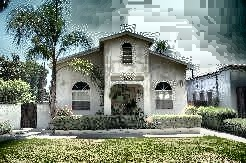
\includegraphics[width=0.45\textwidth]{./Figures/calhouse_234/1-resultado.jpg}
    }
%        \caption{Imagen Original. $\mathscr{H_Y}=0.207231$. $SSIM_R=1$. $SSIM_G=1$. $SSIM_B=1$}
\end{subfigure}
    ~ %add desired spacing between images. e. g. ~. \quad. \qquad. \hfill etc. 
      %(or a blank line to force the subfigure onto a new line)
      \begin{subfigure}[ID=1]{
      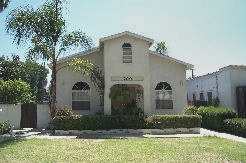
\includegraphics[width=0.45\textwidth]{./Figures/calhouse_234/2-resultado.jpg}   
      }
    %\begin{subfigure}[t]{0.45\textwidth}
%        \caption{Enhanced Image. $\mathscr{H_Y}=0.611275$. $SSIM_R=0.00897331$. $SSIM_G=0.00823064$. $SSIM_B=0.00851013$}
\end{subfigure}
    ~ %add desired spacing between images. e. g. ~. \quad. \qquad. \hfill etc. 
    %(or a blank line to force the subfigure onto a new line)
    \begin{subfigure}[ID=23]{
    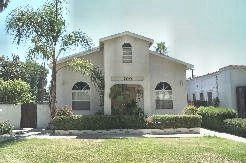
\includegraphics[width=0.45\textwidth]{./Figures/calhouse_234/51-resultado.jpg}
    }
    % \begin{subfigure}[t]{0.45\textwidth}
%        \caption{Enhanced Image.  $\mathscr{H_Y}=0.0350595$. $SSIM_R=0.416776$. $SSIM_G=0.403636$. $SSIM_B=0.417654$}
\end{subfigure} 
\begin{subfigure}[ID=24]{
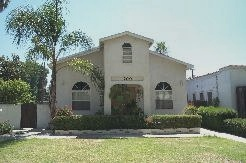
\includegraphics[width=0.45\textwidth]{./Figures/calhouse_234/59-resultado.jpg}
}
    % \begin{subfigure}[t]{0.45\textwidth}
        %\caption{Enhanced Image using \cite{morepso}. $\mathscr{H_Y}=0.788927$. $SSIM_R=0.000204143$. $SSIM_G=0.0000526475$. $SSIM_B=0.0000518143$}
        % \label{fig:calhouse23129}
        \end{subfigure}
    ~ %add desired spacing between images. e. g. ~. \quad. \qquad. \hfill etc. 
    %(or a blank line to force the subfigure onto a new line)
    \begin{subfigure}[ID=56]{
    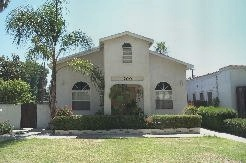
\includegraphics[width=0.45\textwidth]{./Figures/calhouse_234/60-resultado.jpg}
    }
    % \begin{subfigure}[t]{0.45\textwidth}
%        \caption{Enhanced Image.  $\mathscr{H_Y}=0.0350595$. $SSIM_R=0.416776$. $SSIM_G=0.403636$. $SSIM_B=0.417654$}
% \label{fig:calhouse231102}
\end{subfigure} 
\begin{subfigure}[Imagen Original]{
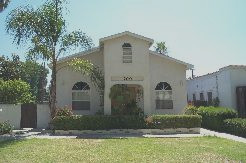
\includegraphics[width=0.45\textwidth]{./Figures/calhouse_234/calhouse_234.jpg}
}
    % \begin{subfigure}[t]{0.45\textwidth}
        %\caption{Enhanced Image using \cite{morepso}. $\mathscr{H_Y}=0.788927$. $SSIM_R=0.000204143$. $SSIM_G=0.0000526475$. $SSIM_B=0.0000518143$}
        % \label{fig:calhouse233orig}
        \end{subfigure}
        \caption{Imágenes visualmente relevantes obtenidas mediante $CMOPSO-CLAHE$. Las variables y decisión y métricas de las imágenes se muestran en la tabla \ref{tab:calhouse_234}.}
        \label{fig:anexocalhouse234}
        \end{figure}

        \begin{figure}[H]
        \centering
        %\begin{subfigure}[Gráfica de Frente Pareto para las soluciones no dominadas de \texttt{calhouse_231.jpg}]{
        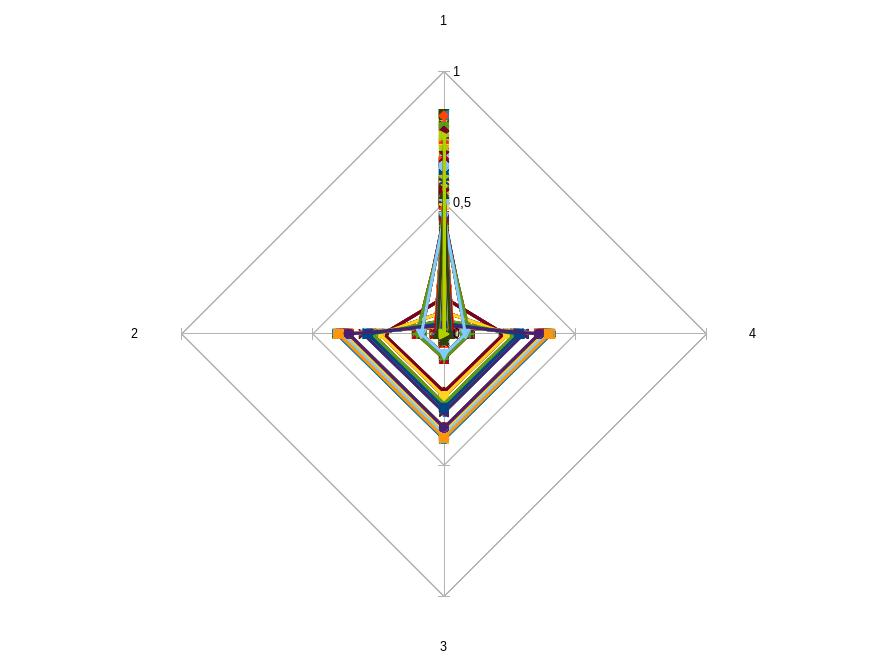
\includegraphics[width=\textwidth]{./Figures/calhouse_234/calhouse_234_2.jpg}
        %}
        %\end{subfigure}
        \caption{Frente pareto que contrasta los objetivos de las soluciones no dominadas. para los resultados de imágenes que se muestran en la tabla \ref{tab:calhouse_234}.}
        \label{fig:calhouse2342fp}
        \end{figure}


\section{Imagen de prueba \texttt{calhouse\_234.jpg}}

%calhouse 234
\scriptsize
\begin{longtable}{|c|c|c|c|c|c|c|c|}
% \centering
%\begin{tabular}
\hline
ID & $\mathscr{R}_x$ & $\mathscr{R}_y$ & $\mathscr{C}$ & $f_1(I.\vv{x})$ & $f_2(I.\vv{x})$ & $f_3(I.\vv{x})$ & $f_4(I.\vv{x})$ \\
2979 & 3 & 3 & 0.812519298752 & 0.511109 & 0.0287218 & 0.0274117 & 0.0284403 \\
2980 & 4 & 12 & 0 & 0.0276203 & 0.49051 & 0.486184 & 0.493034 \\
3091 & 4 & 2 & 0.853706507459 & 0.519737 & 0.027535 & 0.0255765 & 0.0267492 \\
3097 & 11 & 2 & 1 & 0.494054 & 0.034029 & 0.032038 & 0.0331011 \\
3104 & 20 & 3 & 0 & 0.0284328 & 0.402012 & 0.396043 & 0.401629 \\
3123 & 3 & 3 & 0.739306706876 & 0.533226 & 0.024867 & 0.0237548 & 0.0245899 \\
3125 & 2 & 2 & 0.731703535828 & 0.548753 & 0.0229975 & 0.0211807 & 0.0222653 \\
3126 & 3 & 2 & 0.679146848174 & 0.557746 & 0.0203147 & 0.0187927 & 0.0196922 \\
3127 & 2 & 2 & 0.850344549266 & 0.515146 & 0.029663 & 0.0272264 & 0.0286435 \\
3128 & 14 & 2 & 0.632770576643 & 0.58597 & 0.01286 & 0.0122675 & 0.0126854 \\
3129 & 53 & 3 & 0.0906614748552 & 0.41236 & 0.10348 & 0.0946411 & 0.0973958 \\
3130 & 8 & 2 & 0.368264089891 & 0.675727 & 0.00441494 & 0.00421142 & 0.00434589 \\
3131 & 2 & 2 & 0.827779089761 & 0.524632 & 0.0281598 & 0.0258405 & 0.0271833 \\
3132 & 2 & 2 & 0 & 0.138669 & 0.231124 & 0.221532 & 0.228493 \\
3133 & 37 & 4 & 0.488860216273 & 0.445821 & 0.0866204 & 0.0792098 & 0.0816776 \\
3134 & 4 & 2 & 0.255668440752 & 0.730788 & 0.00268251 & 0.00253008 & 0.00260924 \\
3135 & 6 & 2 & 0.912272466777 & 0.496642 & 0.0326795 & 0.0303633 & 0.0316357 \\
3136 & 2 & 2 & 0.0083970078807 & 0.835548 & 0.000142314 & 0.000115598 & 0.000110237 \\
3137 & 3 & 2 & 0.461160630083 & 0.650707 & 0.00852852 & 0.00796836 & 0.00830184 \\
3138 & 3 & 2 & 0.73164070769 & 0.551425 & 0.0215359 & 0.0198995 & 0.0208231 \\
3139 & 4 & 2 & 0.0653533397144 & 0.832464 & 0.000183395 & 0.000143403 & 0.000147903 \\
3140 & 3 & 2 & 0.148486630518 & 0.793742 & 0.000731432 & 0.000664557 & 0.000679274 \\
3141 & 18 & 2 & 0.572302594831 & 0.62303 & 0.00889421 & 0.00828233 & 0.00854233 \\
3142 & 13 & 3 & 0 & 0.0292034 & 0.390222 & 0.383769 & 0.389344 \\
3143 & 9 & 2 & 0.515175605936 & 0.640419 & 0.00871692 & 0.00817691 & 0.00844283 \\
3144 & 10 & 2 & 0.645449480383 & 0.580588 & 0.0168114 & 0.0159317 & 0.0165228 \\
3145 & 24 & 3 & 0 & 0.0277634 & 0.406696 & 0.400567 & 0.40603 \\
3146 & 6 & 2 & 0 & 0.0493283 & 0.277246 & 0.269315 & 0.27368 \\
3147 & 2 & 2 & 0.761261125963 & 0.54257 & 0.0246297 & 0.0226156 & 0.0237819 \\
3148 & 5 & 2 & 0 & 0.0519104 & 0.273498 & 0.265907 & 0.270653 \\
3149 & 2 & 2 & 0.926215684557 & 0.493326 & 0.0350073 & 0.032038 & 0.0337141 \\
3150 & 5 & 3 & 0.907757451731 & 0.507807 & 0.0309136 & 0.0296258 & 0.0305795 \\
3151 & 2 & 2 & 0.729074889936 & 0.553606 & 0.021385 & 0.0196689 & 0.0206698 \\
3152 & 3 & 2 & 0 & 0.0846047 & 0.245215 & 0.237309 & 0.244065 \\
3153 & 3 & 2 & 0.854113478667 & 0.512472 & 0.030045 & 0.027703 & 0.0290506 \\
3154 & 7 & 3 & 0 & 0.0321503 & 0.363205 & 0.357271 & 0.362161 \\
3155 & 24 & 2 & 1 & 0.448877 & 0.0337654 & 0.0325268 & 0.0334449 \\
3156 & 4 & 2 & 0.780918170773 & 0.530471 & 0.0249754 & 0.0230687 & 0.0241613 \\
3157 & 6 & 2 & 0.196390542599 & 0.78611 & 0.000841764 & 0.00080091 & 0.000816869 \\
3158 & 2 & 3 & 0.833866902733 & 0.511989 & 0.0302699 & 0.0285167 & 0.0297871 \\
3159 & 6 & 2 & 0.747192629244 & 0.547824 & 0.0229913 & 0.0213657 & 0.0222196 \\
3160 & 3 & 2 & 0.80975515976 & 0.527355 & 0.0266691 & 0.0245697 & 0.0257519 \\
3161 & 7 & 2 & 0 & 0.0413656 & 0.289774 & 0.282049 & 0.285934 \\
3162 & 3 & 3 & 0.725942475481 & 0.553035 & 0.0211689 & 0.0201818 & 0.0209119 \\
3163 & 2 & 3 & 0.0869925259854 & 0.831217 & 0.000254231 & 0.000202246 & 0.000220666 \\
3164 & 3 & 2 & 0.101165992212 & 0.829471 & 0.000258416 & 0.000220973 & 0.000231715 \\
3165 & 6 & 2 & 0.846937821181 & 0.518807 & 0.027765 & 0.0259249 & 0.0270216 \\
3166 & 3 & 2 & 0.305290000047 & 0.710093 & 0.00364066 & 0.0034385 & 0.00355669 \\
3167 & 11 & 2 & 0 & 0.0396638 & 0.306313 & 0.297956 & 0.302221 \\
3168 & 7 & 2 & 0.219179192327 & 0.773407 & 0.00121588 & 0.00114323 & 0.00117378 \\
3169 & 5 & 2 & 0.227660930211 & 0.738358 & 0.00171736 & 0.0016441 & 0.00168794 \\
3170 & 26 & 6 & 0.511796994819 & 0.445776 & 0.0921568 & 0.0871899 & 0.0896835 \\
3171 & 3 & 2 & 0.225128485738 & 0.755389 & 0.00142469 & 0.00136878 & 0.00139945 \\
3172 & 2 & 3 & 0.0112353502775 & 0.836594 & 0.000146742 & 0.000117982 & 0.000110062 \\
3173 & 17 & 2 & 0.73226869704 & 0.574325 & 0.0167192 & 0.0159348 & 0.0164249 \\
3174 & 11 & 3 & 0 & 0.0296307 & 0.381211 & 0.374829 & 0.380207 \\
3175 & 4 & 2 & 0.863033788718 & 0.502655 & 0.0311266 & 0.0287067 & 0.03005 \\
3176 & 14 & 2 & 0.937018260677 & 0.502234 & 0.0314391 & 0.0298899 & 0.0308901 \\
3177 & 3 & 3 & 0.578272628825 & 0.582351 & 0.0151525 & 0.0144716 & 0.0149766 \\
3178 & 6 & 2 & 0.682234104882 & 0.564373 & 0.0195332 & 0.0183163 & 0.019096 \\
3179 & 18 & 2 & 0.783902002406 & 0.533793 & 0.0238637 & 0.022623 & 0.0232914 \\
3180 & 4 & 3 & 0.403556720027 & 0.65922 & 0.00689137 & 0.00665012 & 0.00686885 \\
3181 & 2 & 3 & 0.885217278433 & 0.492458 & 0.0341363 & 0.0321934 & 0.0336531 \\
3182 & 11 & 2 & 0.317936251338 & 0.723333 & 0.00331185 & 0.00315496 & 0.00324682 \\
3183 & 15 & 2 & 0.5 & 0.666303 & 0.00554846 & 0.00524035 & 0.00540413 \\
3184 & 12 & 2 & 0.522610271857 & 0.601996 & 0.0103419 & 0.00983332 & 0.010186 \\
3185 & 11 & 2 & 0.95 & 0.513048 & 0.0288726 & 0.0272513 & 0.0282724 \\
3186 & 3 & 3 & 0.656165744218 & 0.571977 & 0.0180757 & 0.0172713 & 0.0179017 \\
3187 & 13 & 2 & 0.956428228721 & 0.524695 & 0.0260812 & 0.024745 & 0.0255167 \\
\hline
\multicolumn{8}{|c|}{\textbf{Tiempos de ejecución:} \texttt{real:69m51.735s, user:207m51.484s, sys:94m33.030s}}\\  \hline
% \end{tabular}
\caption{Resultados no dominados para la imagen de prueba \texttt{calhouse\_234.jpg}}
\label{tab:calhouse_234}
\end{longtable}
\normalsize

\begin{figure}[H]
\centering
    %\begin{subfigure}[t]{0.45\textwidth}
    \begin{subfigure}[ID=0]{
    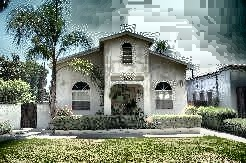
\includegraphics[width=0.45\textwidth]{./Figures/calhouse_234/1-resultado.jpg}
    }
%        \caption{Imagen Original. $\mathscr{H_Y}=0.207231$. $SSIM_R=1$. $SSIM_G=1$. $SSIM_B=1$}
\end{subfigure}
    ~ %add desired spacing between images. e. g. ~. \quad. \qquad. \hfill etc. 
      %(or a blank line to force the subfigure onto a new line)
      \begin{subfigure}[ID=1]{
      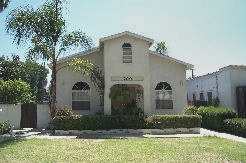
\includegraphics[width=0.45\textwidth]{./Figures/calhouse_234/2-resultado.jpg}   
      }
    %\begin{subfigure}[t]{0.45\textwidth}
%        \caption{Enhanced Image. $\mathscr{H_Y}=0.611275$. $SSIM_R=0.00897331$. $SSIM_G=0.00823064$. $SSIM_B=0.00851013$}
\end{subfigure}
    ~ %add desired spacing between images. e. g. ~. \quad. \qquad. \hfill etc. 
    %(or a blank line to force the subfigure onto a new line)
    \begin{subfigure}[ID=23]{
    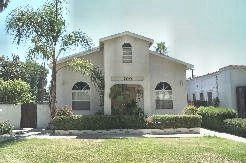
\includegraphics[width=0.45\textwidth]{./Figures/calhouse_234/51-resultado.jpg}
    }
    % \begin{subfigure}[t]{0.45\textwidth}
%        \caption{Enhanced Image.  $\mathscr{H_Y}=0.0350595$. $SSIM_R=0.416776$. $SSIM_G=0.403636$. $SSIM_B=0.417654$}
\end{subfigure} 
\begin{subfigure}[ID=24]{
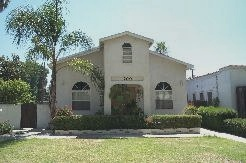
\includegraphics[width=0.45\textwidth]{./Figures/calhouse_234/59-resultado.jpg}
}
    % \begin{subfigure}[t]{0.45\textwidth}
        %\caption{Enhanced Image using \cite{morepso}. $\mathscr{H_Y}=0.788927$. $SSIM_R=0.000204143$. $SSIM_G=0.0000526475$. $SSIM_B=0.0000518143$}
        % \label{fig:calhouse23129}
        \end{subfigure}
    ~ %add desired spacing between images. e. g. ~. \quad. \qquad. \hfill etc. 
    %(or a blank line to force the subfigure onto a new line)
    \begin{subfigure}[ID=56]{
    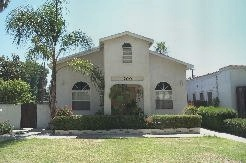
\includegraphics[width=0.45\textwidth]{./Figures/calhouse_234/60-resultado.jpg}
    }
    % \begin{subfigure}[t]{0.45\textwidth}
%        \caption{Enhanced Image.  $\mathscr{H_Y}=0.0350595$. $SSIM_R=0.416776$. $SSIM_G=0.403636$. $SSIM_B=0.417654$}
% \label{fig:calhouse231102}
\end{subfigure} 
\begin{subfigure}[Imagen Original]{
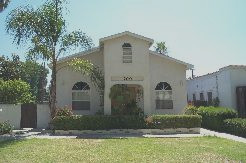
\includegraphics[width=0.45\textwidth]{./Figures/calhouse_234/calhouse_234.jpg}
}
    % \begin{subfigure}[t]{0.45\textwidth}
        %\caption{Enhanced Image using \cite{morepso}. $\mathscr{H_Y}=0.788927$. $SSIM_R=0.000204143$. $SSIM_G=0.0000526475$. $SSIM_B=0.0000518143$}
        % \label{fig:calhouse233orig}
        \end{subfigure}
        \caption{Imágenes visualmente relevantes obtenidas mediante $CMOPSO-CLAHE$. Las variables y decisión y métricas de las imágenes se muestran en la tabla \ref{tab:calhouse_234}.}
        \label{fig:anexocalhouse234}
        \end{figure}

        \begin{figure}[H]
        \centering
        %\begin{subfigure}[Gráfica de Frente Pareto para las soluciones no dominadas de \texttt{calhouse_231.jpg}]{
        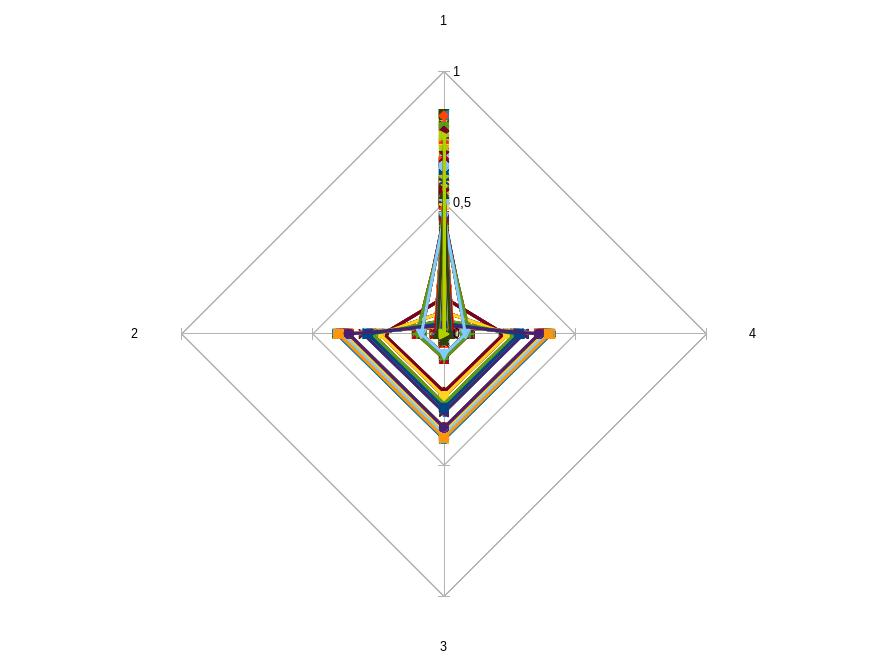
\includegraphics[width=\textwidth]{./Figures/calhouse_234/calhouse_234_2.jpg}
        %}
        %\end{subfigure}
        \caption{Frente pareto que contrasta los objetivos de las soluciones no dominadas. para los resultados de imágenes que se muestran en la tabla \ref{tab:calhouse_234}.}
        \label{fig:calhouse2342fp}
        
% \begin{table}[H]
% \centering
% \caption{Promedios de los tiempos de ejecución de algoritmo HE para las imágenes en escala de grises.}
% \label{tabla22}
% \begin{tabular}{|c|c|}
% \hline
% \begin{tabular}[c]{@{}c@{}}Nº de \\ ejecución\end{tabular} & \begin{tabular}[c]{@{}c@{}}t\\ (ms)\end{tabular} \\ \hline
% 1                                                          & 1.145                                            \\
% 2                                                          & 0.945                                            \\
% 3                                                          & 0.97                                             \\
% 4                                                          & 0.925                                            \\
% 5                                                          & 0.95                                             \\ \hline
% Promedio                                                   & \textbf{0.987}                                   \\ \hline
% \end{tabular}
% \end{table}


% En la Tabla \ref{tabla23} se muestran los promedios de los tiempos de ejecución del algoritmo MMCE para las imágenes en escala de grises.

% % Please add the following required packages to your document preamble:
% % \usepackage{multirow}
% \begin{table}[H]
% 	\centering
% 	\caption{Promedios de los tiempos de ejecución del algoritmo MMCE para las imágenes en escala de grises.}
% 	\label{tabla23}
% 	\begin{tabular}{|c|c|c|c|c|c|c|}
% 		\hline
% 		\multirow{2}{*}{Iter. (n)} & \multicolumn{5}{c|}{Nº de ejeciciones para el algoritmo MMCE} & \multirow{2}{*}{\begin{tabular}[c]{@{}c@{}}Promedios\\ t(ms)\end{tabular}} \\ \cline{2-6}
% 		& 1           & 2          & 3         & 4         & 5          &                                                                            \\ \hline
% 		1                          & 64.265      & 62.625     & 61.61     & 62.285    & 62.295     & \textbf{62.616}                                                            \\
% 		2                          & 165.805     & 171.24     & 169.655   & 170.515   & 170.295    & \textbf{169.502}                                                           \\
% 		3                          & 327.975     & 334.19     & 334.75    & 332.045   & 333.275    & \textbf{332.447}                                                           \\
% 		4                          & 564.035     & 574.15     & 571.185   & 573.45    & 568.735    & \textbf{570.311}                                                           \\
% 		5                          & 975.845     & 972.035    & 979.205   & 968.975   & 986.805    & \textbf{976.573}                                                           \\
% 		6                          & 1454.415    & 1471.145   & 1449.78   & 1452.97   & 1463.74    & \textbf{1458.41}                                                           \\
% 		7                          & 2037.11     & 2032.775   & 2041.54   & 2029.07   & 2038.735   & \textbf{2035.846}                                                          \\ \hline
% 	\end{tabular}
% \end{table}


% En la Tabla \ref{tabla24} se muestran los promedios de los tiempos de ejecución del algoritmo propuesto para las imágenes en escala de grises.

% % Please add the following required packages to your document preamble:
% % \usepackage{multirow}
% \begin{table}[H]
% 	\centering
% 	\caption{Promedios de los tiempos de ejecución del algoritmo propuesto para las imágenes en escala de grises.}
% 	\label{tabla24}
% 	\begin{tabular}{|c|c|c|c|c|c|c|}
% 		\hline
% 		\multirow{2}{*}{Iter. (n)} & \multicolumn{5}{c|}{Nº de ejeciciones para el algoritmo propuesto} & \multirow{2}{*}{\begin{tabular}[c]{@{}c@{}}Promedios \\ t(ms)\end{tabular}} \\ \cline{2-6}
% 		& 1            & 2           & 3           & 4          & 5          &                                                                             \\ \hline
% 		1                          & 62.105       & 63.055      & 61.99       & 62.445     & 62.955     & 62.51                                                                       \\
% 		2                          & 166.74       & 169.645     & 168.34      & 168.435    & 169.34     & 168.5                                                                       \\
% 		3                          & 327.175      & 332.58      & 331.765     & 332.755    & 331.52     & 331.159                                                                     \\
% 		4                          & 565.245      & 576.84      & 574.47      & 573.6      & 572.15     & 572.461                                                                     \\
% 		5                          & 976.57       & 973.22      & 968.35      & 970.245    & 975.26     & 972.729                                                                     \\
% 		6                          & 1463.175     & 1474.82     & 1458.765    & 1459.83    & 1470.06    & 1465.33                                                                     \\
% 		7                          & 2047.435     & 2040.82     & 2041.915    & 2039.95    & 2044.16    & 2042.856                                                                    \\ \hline
% 	\end{tabular}
% \end{table}

